% ==== Foundations ====
\section{Foundations}

\begin{frame}{LLVM}
  \begin{itemize}
    \itemsep=1ex

  \item %\includegraphics[height=\baselineskip]{img/llvm.png}
    LLVM and clang to the rescue!
    \begin{center}
      
\includegraphics[width=1in]{img/LLVMWyvernSmall.png}
    \end{center}

  \item LLVM gives all the infrastructure required to build a compiler
    \begin{itemize}
    \item Basic data structures, e.g. \texttt{llvm::SmallVector}, or \texttt{llvm::Twine}
    \item An intermediate representation (LLVM IR)
    \item Lowering to machine code for many targets: x86\_64, ARM7, AArch64, RISC-V, etc.
    \item Machine-dependent and machine-independent optimization passes
    \item Generation of debug information
    \end{itemize}
  \end{itemize}

  \only<2->{
    \begin{tikzpicture}[remember picture,overlay]
      \node[anchor=east,opacity=.9] at ($(current page.east)+(-.85in,-1in)$) {\tikz{
          \StickyNotePi[0.6in]{\footnotesize And more!  See \url{\llvmURL}.}[1.9in]%
      }};
    \end{tikzpicture}
  }

  \only<3->{
    \begin{tikzpicture}[remember picture,overlay]
      \node[draw,fill=white] at (current page.center) {\tikz[start chain=c going right,node distance=11pt,
  every node/.style={font=\scriptsize},
  every on chain/.style={join=by ->},
  rect/.style={draw,fill=white,text width=1in,align=center,minimum height=22pt,inner sep=1pt},
  container/.style={draw,densely dotted,top color=black!6,bottom color=white,rounded corners}]{

  \begin{scope}[every node/.append style=on chain]
    \path node(test_cpp) {test.cpp}
    % Frontend
    node(lexer)[rect] {Lexical analysis\\ (Lexer)}
    node(parser)[rect] {Syntactic analysis\\ (Parser)}
    node(sema)[rect] {Semantic analysis\\ (Sema)}
    node(IR)[rect] {Generate IR}
    % Backend
    node(optI)[continue chain=c going below,node distance=42pt,rect] {Arch-independent optimization}
    node(optD)[continue chain=c going left,node distance=11pt,rect] {Arch-dependent optimization}
    node(codegen)[rect] {Code generation}
    %
    node(test_0) {test.o};
  \end{scope}

  % Symbol tables and AST
  \draw[<->] (parser) -- ++(up:30pt) node(symtabs)[at end,anchor=south,label={right:Symbol tables}]{\tikz\foreach \i
    in {0pt,-2pt,-4pt} \node[inner sep=4pt,draw,fill=white,xshift=\i,yshift=\i]{};};
  \draw[<->] (sema) -- ++(up:30pt) node(ast)[at end,anchor=south,label={right:AST}]{\tikz\graph[tree layout,level distance=4pt,sibling distance=4pt,nodes={circle,inner sep=1.5pt,as=,fill=black}]{ a -- { b, c }};};

  % Draw fronend and backend rectangles
  \begin{pgfonlayer}{background}
    \path node(fe)[container,inner xsep=4pt,inner ysep=3pt,yshift=-3pt,fit={(lexer)(parser)(sema)(IR)(ast)}]{}
          node(be)[container,inner xsep=4pt,inner ysep=12pt,yshift=6pt,fit={(optI)(optD)(codegen)}]{};

    \foreach \i/\j in {fe/{Compiler frontend},be/{Compiler backend (LLVM)}}
      \node[font={\scriptsize\bfseries},above=0pt of \i.north west,anchor=north west]{\j};
  \end{pgfonlayer}

}
};
    \end{tikzpicture}
  }
\end{frame}

\begin{frame}[fragile]{LLVM IR}
  % == PART 1
  \begin{onlyenv}<1>
   \begin{itemize}
      \itemsep=1ex

    \item LLVM IR may have 3 different representations: \textbf{in-memory} structures, assembly-like \textbf{plain-text}, or \textbf{serialized} form
    \item Let's play a bit to build the LLVM IR for a simple function!
    \end{itemize}
  \end{onlyenv}

  % == PART 2
  \begin{onlyenv}<2->
    \begin{lstlisting}[style=c++]
LLVMContext C;
auto builder = std::make_unique<IRBuilder<>>(C);
auto M = std::make_unique<Module>("main", C);

auto i32 = builder->getInt32Ty();
auto funcTy = FunctionType::get(`\lsthl{i32, \{i32, i32\}}`, /*isVarArg=*/false);
auto func = Function::Create(funcTy, GlobalValue::LinkageTypes::ExternalLinkage, `\lsthl{"func"}`, *M);
auto BB = BasicBlock::Create(C, "entry", func);
builder->SetInsertPoint(BB);
auto addVal = builder->`\lsthl{CreateAdd}`(func->getArg(0), func->getArg(1));
builder->`\lsthl{CreateRet}`(addVal);
M->print(errs(), /*AAW=*/nullptr);
    \end{lstlisting}
  \end{onlyenv}

  \begin{onlyenv}<3->
    \begin{tikzpicture}[remember picture,overlay]
      \node[draw,fill=white,font={\ttfamily\footnotesize}] at ($(current page.east)+(-2in,0pt)$) {
            \begin{minipage}{2.5in}
; ModuleID = 'main'\\
source\_filename = "main"\\
\\
{\bfseries define i32} \@func({\bfseries i32} \%0, {\bfseries i32} \%1) \{\\
entry:\\
\rule{20pt}{0pt}\%2 = {\bfseries add i32} \%0, \%1\\
\rule{20pt}{0pt}{\bfseries ret i32} \%2\\
\}\\
            \end{minipage}
      };
    \end{tikzpicture}
  \end{onlyenv}

\end{frame}

\begin{frame}[fragile]{LLVM JIT / ORC}
  LLVM can also JIT IR to current target's machine code\ldots{}%
  \footnote{Full example: \url{https://github.com/jalopezg-git/slides-using_stdcpp_2014/blob/master/code/llvm-ir.cpp}}

  \vfill
  \begin{lstlisting}[style=c++]
int main(int argc, char *argv[]) {
  using namespace llvm;
  InitializeNativeTarget();
  InitializeNativeTargetAsmPrinter();

  /* CREATE IR AS IN PREVIOUS SLIDE */
  
  auto EE = EngineBuilder(std::move(M)).setEngineKind(llvm::EngineKind::JIT).create();

  using FuncPtr_t = uint32_t (*)(uint32_t, uint32_t);
  auto pFunc = (FuncPtr_t)EE->getFunctionAddress("func");
  auto ret = `\lsthl{pFunc(42, 7)}`;
  errs() << "\nfunc() returned " << ret << "\n";

  return 0;
}
  \end{lstlisting}

  \only<2->{
    \begin{tikzpicture}[remember picture,overlay]
      \node[anchor=east,opacity=.9] at ($(current page.east)+(-.85in,-1in)$) {\tikz{\StickyNotePi[0.6in]{
            {\ttfamily func() returned 49}
          }[1.9in]%
      }};
    \end{tikzpicture}
  }
\end{frame}

\begin{frame}[fragile]{Clang as a library}
  % == PART 1
  \begin{onlyenv}<1>
    \begin{itemize}
      \itemsep=1ex

    \item Clang is basically a frontend that parses C / C++ / ObjectiveC and generates LLVM IR, i.e.
      \begin{itemize}
      \item It does lexical / gramatical /  semantic analysis on the source code + builds an AST
      \item LLVM takes over from there
      \end{itemize}

    \item E.g., the simple code\ldots{}
      \lstinputlisting[style=c++]{code/puts-simple.c}
    \end{itemize}
  \end{onlyenv}

  % == PART 2
  \begin{onlyenv}<2>
    \lstinputlisting[style=c++]{code/puts-simple.c}
    \vfill

    Has AST representation\footnote{Get this with \texttt{clang -c -Xclang -ast-dump -o /dev/stdout input.c}}
    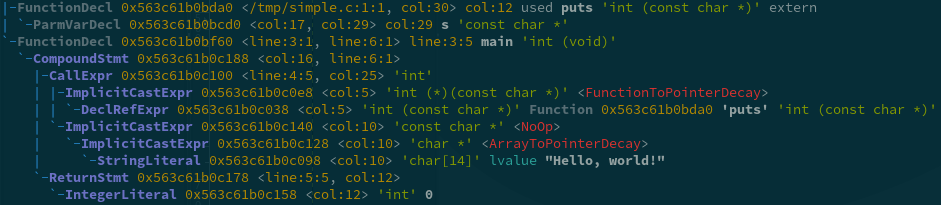
\includegraphics[width=\textwidth]{img/clang-ast.png}
  \end{onlyenv}

  % == PART 3
  \begin{onlyenv}<3>
    \lstinputlisting[style=c++]{code/puts-simple.c}
    \vfill

    And LLVM IR representation\footnote{Get this with \texttt{clang -S -emit-llvm -o /dev/stdout input.c}}
    \begin{lstlisting}[language=llvm,basicstyle={\ttfamily\fontsize{6.5}{6.5}\selectfont}]
; ModuleID = '/tmp/simple.c'
source_filename = "/tmp/simple.c"
target datalayout = "e-m:e-p270:32:32-p271:32:32-p272:64:64-i64:64-f80:128-n8:16:32:64-S128"
target triple = "x86_64-pc-linux-gnu"

@.str = private unnamed_addr constant [14 x i8] c"Hello, world!\00", align 1

; Function Attrs: nofree nounwind sspstrong uwtable
define dso_local i32 @main() local_unnamed_addr #0 {
  %1 = tail call i32 @puts(ptr noundef nonnull dereferenceable(1) @.str)
  ret i32 0
}

; Function Attrs: nofree nounwind
declare noundef i32 @puts(ptr nocapture noundef readonly) local_unnamed_addr #1
    \end{lstlisting}
  \end{onlyenv}
\end{frame}

\begin{frame}{Clang as a library}
  \begin{itemize}
    \itemsep=1ex

  \item And it offers libTooling, libclang-cpp, and libclang!

  \item Meaning we can mostly reuse this%
    \footnote{Modulo some patches required to clang.}%
    and only write a layer on top that does ``impedance matching'' between ISO and interpreted C++
  \end{itemize}
\end{frame}
